% This is "aamas2015_sample.tex", a revised version of aamas2014_sample.tex
% This file should be compiled with "aamas2015.cls" 
% This example file demonstrates the use of the 'aamas2015.cls'
% LaTeX2e document class file. It is intended for those submitting
% articles to the AAMAS-2015 conference. This file is based on
% the sig-alternate.tex example file.
% The 'sig-alternate.cls' file of ACM will produce a similar-looking,
% albeit, 'tighter' paper resulting in, invariably, fewer pages
% than the original ACM style.
%
% ----------------------------------------------------------------------------------------------------------------
% This .tex file (and associated .cls ) produces:
%       1) The Permission Statement
%       2) The Conference (location) Info information
%       3) The Copyright Line with AAMAS data
%       4) NO page numbers
%
% as against the acm_proc_article-sp.cls file which
% DOES NOT produce 1) through 3) above.
%
% Using 'aamas2015.cls' you don't have control
% from within the source .tex file, over both the CopyrightYear
% (defaulted to 20XX) and the IFAAMAS Copyright Data
% (defaulted to X-XXXXX-XX-X/XX/XX).
% These information will be overwritten by fixed AAMAS 2015  information
% in the style files - it is NOT as you are used to with ACM style files.
%
% ---------------------------------------------------------------------------------------------------------------
% This .tex source is an example which *does* use
% the .bib file (from which the .bbl file is produced).
% REMEMBER HOWEVER: After having produced the .bbl file,
% and prior to final submission, you *NEED* to 'insert'
% your .bbl file into your source .tex file so as to provide
% ONE 'self-contained' source file.
%


\documentclass{aamas2015}

% if you are using PDF LaTeX and you cannot find a way for producing
% letter, the following explicit settings may help
\usepackage{times}
\usepackage{url}
\usepackage{helvet}
\usepackage{courier}
\usepackage{graphicx}
\usepackage{subfigure}
%\usepackage[lined,boxed,commentsnumbered, ruled]{algorithm2e}
\usepackage{algorithm}
\usepackage{algorithmic}
\usepackage{balance}
\usepackage{slashbox}

\usepackage{xcolor}
\newtheorem{theorem}{Theorem}%[section]
\newtheorem{proposition}{Proposition}
\newtheorem{definition}{Definition}
\newtheorem{lemma}{Lemma}
\newtheorem{property}{Property}
\frenchspacing
\pdfpagewidth=8.5truein
\pdfpageheight=11truein

\begin{document}



\title{Optimizing water right trading assignments at Shiyang River basin}

% AUTHORS


% For initial submission, do not give author names, but the
% tracking number, instead, as the review process is blind.

% You need the command \numberofauthors to handle the 'placement
% and alignment' of the authors beneath the title.
%
% For aesthetic reasons, we recommend 'three authors at a time'
% i.e. three 'name/affiliation blocks' be placed beneath the title.
%
% NOTE: You are NOT restricted in how many 'rows' of
% "name/affiliations" may appear. We just ask that you restrict
% the number of 'columns' to three.
%
% Because of the available 'opening page real-estate'
% we ask you to refrain from putting more than six authors
% (two rows with three columns) beneath the article title.
% More than six makes the first-page appear very cluttered indeed.
%
% Use the \alignauthor commands to handle the names
% and affiliations for an 'aesthetic maximum' of six authors.
% Add names, affiliations, addresses for
% the seventh etc. author(s) as the argument for the
% \additionalauthors command.
% These 'additional authors' will be output/set for you
% without further effort on your part as the last section in
% the body of your article BEFORE References or any Appendices.

%\numberofauthors{8} %  in this sample file, there are a *total*
% of EIGHT authors. SIX appear on the 'first-page' (for formatting
% reasons) and the remaining two appear in the \additionalauthors section.
%

\numberofauthors{1}

\author{
% You can go ahead and credit any number of authors here,
% e.g. one 'row of three' or two rows (consisting of one row of three
% and a second row of one, two or three).
%
% The command \alignauthor (no curly braces needed) should
% precede each author name, affiliation/snail-mail address and
% e-mail address. Additionally, tag each line of
% affiliation/address with \affaddr, and tag the
% e-mail address with \email.
% 1st. author
\alignauthor
Paper 76
%Ben Trovato\titlenote{Dr.~Trovato insisted his name be first.}\\
%       \affaddr{Institute for Clarity in Documentation}\\
%       \affaddr{1932 Wallamaloo Lane}\\
%       \affaddr{Wallamaloo, New Zealand}\\
%       \email{trovato@corporation.com}
% 2nd. author
%\alignauthor
%G.K.M. Tobin\titlenote{The secretary disavows any knowledge of this author's actions.}\\
%       \affaddr{Institute for Clarity in Documentation}\\
%       \affaddr{P.O. Box 1212}\\
%       \affaddr{Dublin, Ohio 43017-6221}\\
%       \email{webmaster@marysville-ohio.com}
% 3rd. author
%\alignauthor Lars Th{\o}rv{\"a}ld\titlenote{This author is the one who did all the really hard work.}\\
%       \affaddr{The Th{\o}rv{\"a}ld Group}\\
%       \affaddr{1 Th{\o}rv{\"a}ld Circle}\\
%       \affaddr{Hekla, Iceland}\\
%       \email{larst@affiliation.org}
}

%\and  % use '\and' if you need 'another row' of author names

% 4th. author
%\alignauthor Lawrence P. Leipuner\\
%       \affaddr{Brookhaven Laboratories}\\
%       \affaddr{Brookhaven National Lab}\\
%       \affaddr{P.O. Box 5000}\\
%       \email{lleipuner@researchlabs.org}

% 5th. author
%\alignauthor Sean Fogarty\\
%       \affaddr{NASA Ames Research Center}\\
%       \affaddr{Moffett Field}\\
%       \affaddr{California 94035}\\
%       \email{fogartys@amesres.org}

% 6th. author
%\alignauthor Charles Palmer\\
%       \affaddr{Palmer Research Laboratories}\\
%      \affaddr{8600 Datapoint Drive}\\
%       \affaddr{San Antonio, Texas 78229}\\
%       \email{cpalmer@prl.com}

%\and

%% 7th. author
%\alignauthor Lawrence P. Leipuner\\
%       \affaddr{Brookhaven Laboratories}\\
%       \affaddr{Brookhaven National Lab}\\
%       \affaddr{P.O. Box 5000}\\
%       \email{lleipuner@researchlabs.org}

%% 8th. author
%\alignauthor Sean Fogarty\\
%       \affaddr{NASA Ames Research Center}\\
%       \affaddr{Moffett Field}\\
%       \affaddr{California 94035}\\
%       \email{fogartys@amesres.org}

%% 9th. author
%\alignauthor Charles Palmer\\
%       \affaddr{Palmer Research Laboratories}\\
%       \affaddr{8600 Datapoint Drive}\\
%       \affaddr{San Antonio, Texas 78229}\\
%       \email{cpalmer@prl.com}

%}

%% There's nothing stopping you putting the seventh, eighth, etc.
%% author on the opening page (as the 'third row') but we ask,
%% for aesthetic reasons that you place these 'additional authors'
%% in the \additional authors block, viz.
%\additionalauthors{Additional authors: John Smith (The Th{\o}rv{\"a}ld Group,
%email: {\texttt{jsmith@affiliation.org}}) and Julius P.~Kumquat
%(The Kumquat Consortium, email: {\texttt{jpkumquat@consortium.net}}).}
%\date{30 July 1999}
%% Just remember to make sure that the TOTAL number of authors
%% is the number that will appear on the first page PLUS the
%% number that will appear in the \additionalauthors section.

\maketitle

\begin{abstract}
Water is an indispensable public source. In arid regions, it is also a scarce resource. To address ``the tragedy of the common'', most governments operate via a {\em water right system}. The system predicts the demand of each party, allocates water according to the demands and then sets up a marketplace for the parties to trade.

We aim for an efficient water right assignment for the Shiyang River Basin, a pilot water right market in China. Unique features in this region render our problem certain interesting constraints. First, the problem can be viewed as a double-sided market where agents are located on a geographically constrained graph. Second, trading volume between each pair cannot be too small to cover certain costs, including bargaining costs. Third, the price is settled by bargaining between the agents.

As an important part of the design, we investigate the optimal assignment problem both theoretically and experimentally. For the theoretical part, we show that the general computational problem is {\sc NP-hard} and cannot be efficiently approximated ({\sc MAX SNP-hard}). We use a mixed integer program (MIP) to solve the general case. And with independent interest, we propose a polynomial algorithm on line graphs and cycle graphs.

For the experimental part, we develop a data generator for the water right market and show the efficiency of our algorithms on both computation and social welfare.
% For the experimental part, our results confirm that our MIP and its relaxed LP can work particularly well in general graphs at fairly large scale. On the current instance size, the MIP algorithm is even faster than the designated polynomial time algorithms on special graphs such as lines and trees.
\end{abstract}

% Note that the category section should be completed after reference to the ACM Computing Classification Scheme available at
% http://www.acm.org/about/class/1998/.

\category{I.2.11}{Distributed Artificial Intelligence}{Distributed Artificial Intelligence}
\category{J.4}{Social and Behavioral Sciences}{Economics}

%A category including the fourth, optional field follows...
%\category{D.2.8}{Software Engineering}{Metrics}[complexity measures, performance measures]

%General terms should be selected from the following 16 terms: Algorithms, Management, Measurement, Documentation, Performance, Design, Economics, Reliability, Experimentation, Security, Human Factors, Standardization, Languages, Theory, Legal Aspects, Verification.

\terms{Algorithms, Economics, Theory}

%Keywords are your own choice of terms you would like the paper to be indexed by.

\keywords{water right market, dynamic programming, optimization}

\section{Introduction}
Water is one of the most common yet indispensable resources on this planet. In fact, in arid regions, which cover 41\% of the world area, water is also one of the scarcest resources. As a type of public resource, it inevitably suffers from {\em the tragedy of the common}~\cite{Hardin1968}. In China,  it is known that 80\% of the total water resource is consumed in agriculture, 55\% of which are eventually wasted~\cite{liu2007analysis}, partially due to poorly designed institutions. Among others, designing effective {\em water right system} has turned out to be an effective means to address the inefficient usage of water resource~\cite{ostrom2007private}.

\subsection{Water right trading}
A \textit{water right system} specifies the ownership, usage as well as transfer rule of water rights~\cite{scott1995evolution}. In other words, the system specifies how much water each party is allocated, how the water can be used and how it can be transferred to other parties. The last part, water right transfer (aka. water right trading), is crucial to the system since by no means can the system allocates water rights subject to the dynamically changed demands.

\textit{Water right markets}, the marketplaces of water rights trading, are usually modeled and considered as a multi-agent system\cite{Zhao2009,giret2011mas,almajano2012v}. It has been evidenced that water right trading can result in better water ecological environment~\cite{huang2000water}. Many countries, including Australia and the US, have developed water right trading markets~\cite{zhao2003china}. A key difference of China's water market is that water right is not owned by individuals but governments. All the trades are among villages or clubs rather than individuals\cite{Brown2006}. 

This paper aims to optimize the trades allocation for water right trading at Shiyang River Basin, one of the water rights trading pilot areas in China, which is quite arid. It is worth mentioning that, there existed a trading system that manually matches buy and sell orders. The current system is not able to maximize the trading volume or social welfare\footnote{Formally defined in Preliminaries.}. Unlike common markets, water right markets in China meets many featured properties because of the policies in China. \cite{speed2009comparison} compares the advantages of China's and Australia's water right system.

Our survey of the Shiyang River Basin reveals the following unique features that are incorporated in our design.

\begin{enumerate}
	\item Water rights of each two months are firstly assigned to villages each year. That is the water right decide one village owns is the amount of water it can use during the two months.
	\item The trading and the execution afterwards incur considerable costs. Hence, an implicit constraint is that the transaction volume of each trade must be sufficiently large to compensate the cost.
	\item Leaders of villages have more considerations other than money. When the water right is not enough for planting, the leader won't sell them because it incurs the losses of farmers and they may not efficiently reallocate the earnings from trades to the farmers.
	\item Trades between townships suffers bigger obstacles to be approved.
	\item Agents (Villages) prefer to trade with their neighbors. An instant reason is that if they oversell their water right, they can usually buy it back at the same price. 
	\item The water right trading system do not have rights to decide on a trade but only recommend sellers to buyers.
	\item The trading prices of underground water are restricted to be 0.2 yuan per $m^3$ by government since 2013 (Only for agriculture use). And 0.06 for groundwater. Trades between villages are usually for underground water because groundwater has lower marginal cost.
\end{enumerate}

In light of these observations, we model a water right trading market (water market for short) as a directed bipartite graph consisting of a set of buyers and a set of sellers. An arc is oriented from a buyer to a seller if and only if they are geographically connected and the buyer's bid is above the seller's ask. On each arc, there is volume threshold indicating the lowest transaction volume on this arc, if there is any. Each vertex has a price and a capacity that specifies the demand or supply of the vertex.

A trading assignment is simply a feasible {\em flow}. The value for each arc is its trading volume times the price differences on the end vertices. The \textit{social welfare} is the sum of values for all arcs. Our goal is to compute a trading assignment that maximizes (1)  total trading volume; or (2) social welfare.


\textbf{Remark:} The "fixed price" property incentives us to study maximizing trading volume. We note that optimization any of our objectives may cause untruthful reports. However, for (1), manipulation calls for quite a few information and computation; for (2), it is possible to verify whether villages are truthful (with costs) and punish dishonest villages. If most villages are truthful, (2) surely yields a better solution. 

\subsection{Our contribution}
\begin{itemize}
	\item Directly related theoretical results. Denote the problem of maximizing trading volume by {\sc max-volume} and the other by {\sc max-welfare}. Our results can be summarized as follows.
	\begin{itemize}
		\item Without \textit{transaction thresholds}\footnote{A trade is feasible only if the volume of the trade is above the threshold.}, both problems are in P via linear programming
		\item {\sc max-volume} is {\sc NP-hard}.
		\item {\sc max-welfare} is  {\sc max-snp-hard}
		\item {\sc max-welfare} admits a concise MIP formulation
	\end{itemize}
	\item With independent interest, we study the computational complexity on some special graphs and gets the following interesting results.
	\begin{itemize}
		\item {\sc max-welfare} on line graphs or cycle graphs is in P via dynamic programming and linear programming.
		\item {\sc max-welfare} on $k$-connected graphs is {\sc NP-hard}.
%		\item {\sc max-welfare} on integral $k$-connected graphs is in P via dynamic programming
		\item{\sc max-welfare} on binary trees is {\sc NP-hard}.
%		\item {\sc max-welfare} on integral binary trees is in P via dynamic programming
	\end{itemize}
	\item Experimental results
	\begin{itemize}
		\item We design a greedy algorithm to simulate the matching process in the current market. Our results shows that our MIP outperforms the greedy algorithm significantly.
		\item We test the scalability of our MIP algorithm and show that it is still fast on a graph hundreds of nodes, though the problem is actually {\sc NP-hard}.
%		\item We test our designated P algorithms on graphs with special structures. The algorithms run reasonably fast but slower than MIP.
	\end{itemize}
\end{itemize}

\subsection{Additional related work}

Double-sided market has a long history in economical literature (see~\cite{Myerson83,Barbera1995}). The computation problem on double-sided market has also been considered in various settings~\cite{Kalagnanam00,Sandholm01,Sandholm02,Blume09}. Our work differs from them in that we have threshold on arcs and we consider special structures of graphs. Our problem is also related to a variant of the maximum flow problem where each edge has a minimum flow requirement. This version of maximum flow can be solved in polynomial time~\cite{ford2010flows}. The difference is that, in our model, even an edge is labeled with a transaction threshold, the trading volume can still be 0; while in the maximum flow model, this volume has to be above the minimum flow in any feasible solution.

Erfani et al\cite{erfani2014simulating} build a model for water market in England via optimization. Our work is significantly different from that because of policies. Our work is quite involved in computation issues. 
\section{Preliminaries}
A water right trading market can be modeled by a directed bipartite graph $\mathcal{G}=(\mathcal{V},\mathcal{E})$, where
$\mathcal{V}=\mathcal{V_B}\cup \mathcal{V_S}$.
$\mathcal{V_B}$ denotes the set of buyers, while $\mathcal{V_S}$ denotes the set of sellers.
Agent $v_i$ has a price $p_i$ for each unit of water and the maximum amount of water $q_i$ it demands/supplies. Each directed arc $v_iv_j\in \mathcal{E}$ denotes that seller $v_i$ can sell water right to buyer $v_j$. $v_i$ and $v_j$ are connected if and only if three properties must hold in reality:
(1) $v_i$ and $v_j$ are not distant and familiar with each other;
(2) $v_i$ is a seller and $v_j$ is a buyer;
(3) $p_i<p_j$.

The first constraint is particularly interesting as it distinguishes our market from a common marketplace and embed our market with graph properties.

For each arc $v_iv_j$, there is a minimum amount of transaction volume $lb_{ij}$ imposed, if a transaction were to occur between $v_i$ and $v_j$. This transaction threshold ensures that each transaction cover its cost that is not reflected in the current model.

A trading assignment of the market is a {\em flow} from sellers to buyers. We denote the trading volume on $v_iv_j$ by $f_{ij}$. According to local policies, it is always the case that the center shall not specify any trading price but to leave the price bargaining process to the buyer and seller that are involved\footnote{the price is even fixed since 2013. However, we also care about the case without this policy.}. After the bargaining phase, a price $p_{ij}\in [p_i, p_j]$ is derived.

%The price on $v_iv_j$ is $p_{ij}$, satisfying $p_i<p_{ij}<p_j$.
%For each arc $v_iv_j$, it has a transaction threshold on trading volume $lb_{ij}$ only when $f_{ij}>0$.

We aim to optimize two objectives in this paper: trading volume and social welfare.
%Our objective used in this paper has two versions total trading volume and social welfare.
Trading volume is defined to be $VO=\sum_{v_iv_j\in \mathcal{E}}f_{ij}$.
While, social welfare is defined to be
$SW=\sum_{v_i\in \mathcal{V_S}}\sum_{v_iv_j\in \mathcal{E}} f_{ij}*(p_{ij}-p_i)+\sum_{v_i\in \mathcal{V_B}}\sum_{v_jv_i\in \mathcal{E}} f_{ji}*(p_i-p_{ji})$.
$=\sum_{v_iv_j\in \mathcal{E}}f_{ij}*(p_j-p_i)$.

For an instance in which the price difference between any buyer and seller are the same, social welfare is reduced to trading volume. Therefore, maximizing social welfare is a harder problem than maximizing trading volume.



To sum up, a feasible trading assignment satisfies the following constraints:
\begin{itemize}
	\item  Transaction threshold constraints: $\forall v_iv_j\in \mathcal{E}$, if $f_{ij}>0$, then $f_{ij}\geq lb_{ij}$.
	\item  Supply/demand feasibility constraints:
	$\forall v_i\in \mathcal{V_S}$, $\sum_{v_iv_j\in \mathcal{E}}f_{ij}\leq q_i$ and
	$\forall  v_i\in \mathcal{V_B}$, $\sum_{v_jv_i\in \mathcal{E}}f_{ji}\leq q_i$
\end{itemize}



\section{Water right trading assignments}
%Nowadays, the water right trading platform can just match sellers with buyers. Agents report their valuation and quantities. The prices and quantities won't be shown to the others. We match pairs according to their reports. Bargaining is performed between themselves. Under this setting, the power of platform is quite limited. We only concern about a better water right assignment in this case.

In this section, we investigate the computation problems for the two objectives: trading volume and social welfare. Denote the problem of maximizing trading volume by {\sc max-volume} and the other by {\sc max-welfare}.
%Our results can be summarized as follows.
%\begin{itemize}
%\item When transaction thresholds are all $0$, both problems are in P.
%\item {\sc max-volume} is {\sc NP-hard}.
%\item {\sc max-welfare} is MAX S{\sc NP-hard}
%\item {\sc max-welfare} admits a nice MIP formulation.
%\item {\sc max-welfare} on line graphs or cycle graphs is in P.
%\item {\sc max-welfare} on $k$-connected graphs is {\sc NP-hard}.
%\item {\sc max-welfare} on integral $k$-connected graphs is in P.
%\item{\sc max-welfare} on binary trees is {\sc NP-hard}.
%\item {\sc max-welfare} on integral binary trees is in P.
%\end{itemize}
%
%We will rationalize these special structures of graphs when we proceed to the specific sections.

\subsection{{\sc max-welfare} without Transaction Thresholds}

In this subsection, we analyze the case where all transaction thresholds are zero. As mentioned, {\sc max-volume} can be regarded as a special case of {\sc max-welfare}. We have the following linear program to solve {\sc max-welfare} in this case.

\begin{algorithm}\label{alg:nai}
	\caption{Linear Program for {\sc max-welfare}}
	Variables: $\forall v_iv_j\in \mathcal{E}$, $f_{ij}\geq 0$.\\
	Maximize: $\sum_{v_iv_j\in \mathcal{E}}f_{ij}*(p_j-p_i) $\\
	Subject to: \\
	\begin{itemize}
		\item $f_{ij}\geq 0$, $ \forall v_iv_j\in \mathcal{E}$\\
		\item $\sum_{v_iv_j\in \mathcal{E}}f_{ij}\leq q_i$ $\forall v_i\in \mathcal{V_S}$\\
		\item $\sum_{v_iv_j\in \mathcal{E}}f_{ij}\leq q_j$ $\forall v_j\in \mathcal{V_B}$\\
	\end{itemize}
\end{algorithm}


%
%Such a linear programming can't ensure trading volumes on edges are big enough to be acceptable.
%As bargaining brings great human costs, we need transaction thresholds on trading volumes such that the benefits from trading can cover the costs.

If needed, we can naturally extend this problem to satisfy that each unit of trading on $v_iv_j$ comes at a certain cost $c_{ij}$.
We only need to change the objective function of Algorithm \ref{alg:nai} to be $\sum_{v_iv_j\in \mathcal{E}'}f_{ij}*(p_j-p_i-c_{ij}) $.
\subsection{Maximizing Total Trading Volume}
As mentioned before, {\sc max-volume} can be regarded as a special case of {\sc max-welfare}.
So, the {\sc np-hardness} of {\sc max-volume} implies the {\sc np-hardness} of {\sc max-welfare}.



In this subsection, we prove the decision version of {\sc max-volume} is {\sc np-complete}, that is, deciding whether the total trading volume can reach a fixed value $x$.

\begin{definition}
	Given a set of $n$ objects $O=\{o_1,o_2,\ldots. o_n\}$, the weight of $o_i$ is $w_i$. The {\sc Partition Problem} is to deciding whether there is a subset $S$ of $O$ satisfying $\sum_{o_i\in S}w_i=\sum_{o_i\in O\setminus S}w_i$. It is a well-known {\sc np-complete} problem
\end{definition}

\begin{theorem}\label{thm:npc1}
	Deciding whether the total trading volume can reach a fixed value $X$ is {\sc NP-complete}.
\end{theorem}

\begin{proof}
Given a solution, we can easily verify whether the total trading volume reaches $x$.
So, this problem is in NP.

Given an instance of {\sc Partition Problem}, $O=\{o_1,o_2,\ldots. o_n\}$,  where $o_i$ has weight $w_i$.
We construct an instance of water market  as follows.
We set $X=\sum_{o_i\in O}w_i$.
The graph of the water market is $\mathcal{G}=(\mathcal{V},\mathcal{E})$.
$\mathcal{V}$ contains $n$ sellers $v_1,v_2,\ldots, v_n$ and two buyers $v_{n+1}$ and $v_{n+2}$
For each seller $v_i$($i=1,2,\ldots,n$), $p_i=0$, $q_i=w_i$.
For each buyer $v_i$($i=n+1$, $n+2$), $p_i=1$, $q_i=X/2$.
$\forall i=1,2,\ldots,n$, $\forall j=n+1,n+2$, $v_iv_j\in \mathcal{E}$ with $lb_{ij}=q_i$.

We claim that the total trading volume can reach $X$ if and only if the {\sc Partition Problem} has a feasible partition.
Given a feasible trading assignment, for $i=1,2,\ldots,n$, $f_{i,n+1}>0$ if and only if we put $o_{i}$ into $S$.
In this way, we have constructed a feasible partition.
Given a feasible partition, for $i=1,2,\ldots n$, if $o_i\in S$, set $f_{i,n+1}=q_i$, $f_{i,n+2}=0$; else set $f_{i,n+2}=q_i$, $f_{i,n+1}=0$.
In this way, we obtain a feasible trading assignments.
Both directions then follow directly.
So a feasible trading assignment corresponds to a feasible partition.
Therefore, we have proved the theorem.
\end{proof}
\subsection{Inapproximability}
In this subsection, we show that {\sc max-welfare} is not even approximatable with $o(1)$ error ratio in polynomial time. We need to introduce a complexity class called {\sc max-snp}~\cite{papadimitriou1991optimization}. It is known that {\sc max-snp-complete} problems do not have polynomial algorithm to achieve an approximation ratio\footnote{the cost of a solution divided by optimal solution}  more than $g$ (unless {\sc P=NP}), where $g$ is a constant less than 1.

Papadimitriou and Yannakakis~\shortcite{papadimitriou1991optimization} list 10 known problems that are {\sc max-snp-complete}, including {\sc max cut}, {\sc max 3-SAT} and {\sc max 2-SAT}.

\begin{theorem}
	{\sc max-welfare} is {\sc max snp-hard}. %In particular, there is no {\sc PTAS} for the problem unless P=NP.
\end{theorem}
\begin{proof}
	Our proof is based on the fact that {\sc max is-3} (maximum independent set with degree of each vertex bounded by 3) is a {\sc max snp-complete} problem~\cite{berman1995approximation}.
	
	Given an instance $I$ of {\sc max is-3} on graph $\mathcal{G}=(\mathcal{V},\mathcal{E})$, we construct an instance $I'$ of water right assignment problem as follows.
	Without loss of generality, $\mathcal{G}$ can be considered connected.
	$\mathcal{G}'=(\mathcal{V}',\mathcal{E}')$  denotes the graph of $I'$.
	For each vertex $v_i\in \mathcal{V}$, seller $a_i$ and buyer $b_i$ are in $\mathcal{V}'$,
	$q_{a_i}=q_{b_i}=|\mathcal{V}|$, $p_{a_i}=0$, $p_{b_i}=1/|\mathcal{V}|$ $a_ib_i\in \mathcal{E}'$ with $lb_{a_ib_i}=|\mathcal{V}|$.
	For each edge $v_iv_j\in \mathcal{E}$, $e_{ij}\in \mathcal{V}'$ denotes a buyer in the graph  with $p_{e_{ij}}=q_{e_{ij}}=1$.
	$a_ie_{ij},a_je_{ij}\in \mathcal{E}'$, $lb_{a_ie_{ij}}=lb_{a_je_{ij}}=1$.
	We have the maximum social welfare $OPT(I')=|\mathcal{E}|+OPT(I)$, where $OPT(I)$ denotes the optimal solution for the {\sc max is-3} instance, $OPT(I')$ denotes the optimal social welfare in the water right assignment problem.
	In fact our instance is constructed for vertex cover problem.
	Given the optimal solution for $I'$, we have that there is an optimal solution where all $e_{ij}$'s are assigned with sellers. In this specific solution, If $a_i$ is assigned to $b_i$, it indicates $v_i$ is not in the minimum vertex cover of $\mathcal{G}$, thus in the maximum independent set.
	
	To finish this proof, we need the so-called $L$-reduction\footnote{described in \cite{papadimitriou1991optimization}}. Specifically for our problem, $c$ denotes a solution for $I$, which can be constructed from a solution $c'$ of $I'$ in polynomial time. If we can prove $OPT(I')\leq \alpha OPT(I)$ and $OPT(I)-c\leq \beta(OPT(I')-c')$ ($\alpha$ and $\beta$ are positive constants), it implies our problem is harder to be approximated.
	
	On the one hand,
	We notice that $|\mathcal{V}'|=|\mathcal{V}|*2+|\mathcal{E}|\leq |\mathcal{V}|*2+|\mathcal{V}|*3/2=3.5|\mathcal{V}|$.
	The size of maximum independent set is at least $|\mathcal{V}|/4$.
	We have $OPT(I')\leq 3.5|\mathcal{E}|\leq 14OPT(I)$.
	
	On the other hand, we claim $OPT(I)-c\leq OPT(I')-c'$.
	Given a solution $s'$ of $I'$ with social welfare $c'$, we can construct a solution $s$ for $I$  with cost $c$ as follows.
	(1) for every unassigned $e_{ij}$, force seller $a_i$ to sells to an amount $e_{ij}$. This step will not decrease social welfare.
	(2) if $a_i$ and $b_i$ are assigned to trade, put $v_i$ into the independent set.
	In this way, we construct a feasible solution for the {\sc  max is-3} problem.
	If step (1) is not performed, $OPT(I)-c=OPT(I')-c'$.
	Since step (1) will not increase $OPT(I')-c'$, so $OPT(I)-c\leq OPT(I')-c'$ holds.
	
	This completes the proof that {max-welfare} is {\sc max snp-hard}.
\end{proof}
\subsection{An mixed integer linear program for  {\sc max-welfare}}

We have already know that {\sc max-welfare} is {\sc NP-hard} (because of the {\sc NP-hardness} of {\sc max-volume}) and cannot be approximated efficiently. However, this difficulty can be resolved, to a certain degree, by a concise formulation of mixed integer linear programming (MIP). We will show in the experiment section that, with faster MIP solvers such as {\sc CPLEX}~\footnote{\url{http://www-01.ibm.com/software/commerce/optimization/cplex-optimizer/}}, we can scale this problem to considerably large instances.

A key observation here is that a flow on any edge is either 0 or no less than the transaction threshold. We can then use a 0/1 indicator to denote the flow be 0 or no less than the transaction threshold.

\begin{algorithm}\label{alg:ilp}
	\caption{Integer Linear Program for {\sc max-welfare}}
	Variables: $\forall v_iv_j\in \mathcal{E}$, $f_{ij}\geq 0$, $x_{ij}\in \{0,1\}$.\\
	Maximize: $\sum_{v_iv_j\in \mathcal{E}}f_{ij}*(p_j-p_i) $\\
	Subject to: \\
	\begin{itemize}
		\item $f_{ij}\geq lb_{ij}*x_{ij}$, $ \forall v_iv_j\in \mathcal{E}$
		\item $f_{ij}\leq q_j*x_{ij}$, $ \forall v_iv_j\in \mathcal{E}$
		\item $\sum_{v_iv_j\in \mathcal{E}}f_{ij}\leq q_i$ $\forall  v_i\in \mathcal{V_S}$\\
		\item $\sum_{v_iv_j\in \mathcal{E}}f_{ij}\leq q_j$ $\forall  v_i\in \mathcal{V_B}$\\
	\end{itemize}
\end{algorithm}


\begin{theorem}\label{thm:ilp}
	Algorithm \ref{alg:ilp} always returns the solution of {\sc max-welfare}
\end{theorem}

%The proof is in the appendix. \textcolor{red}{The general idea is that we use $x_{ij}$ to identify whether there is flow on edge $ij$. The constraints works no matter whether there is flow on an arc $ij$, because when $x_ij$ is different, the constraints differ respectively.}
\begin{proof}
To prove this theorem, we only need to argue that the feasible solution set of this integer linear program is the same as the solution set of {\sc max-welfare}.
This proof is conducted in two directions.

First, we prove that a feasible solution of {\sc max-welfare} is also a feasible solution of this integer linear program.
Given a solution of {\sc max-welfare}, $\forall v_iv_j\in \mathcal{E}$, $f_{ij}=0$ or $f_{ij}\geq lb_{ij}$.
If $f_{ij}=0$, we set $x_{ij}=0$; else, set $x_{ij}=1$.
When $x_{ij}=1$, the first constraint is exactly the transaction threshold constraint and the second can always be satisfied according to supply/demand feasibility constraints of {\sc max-welfare}.
Under such a construction, we have a feasible solution of the integer linear program.
As supply/demand feasibility constraints are hold for a feasible solution, so the last two constraints in the integer linear programming must be satisfied.

Second, given a feasible solution of the integer linear program, it is a feasible solution of {\sc max-welfare}.
We use $f_{ij}$ in the solution as the volume on $v_iv_j$.
The last constraints corresponding to the supply/demand feasibility constraints of {\sc max-welfare}.
$x_{ij}$ only have two possible values $0$ and $1$.
When $x_{ij}=1$, the first constraint becomes $f_{ij}\geq lb_{ij}$, which satisfies the transaction threshold constraints.
When $x_{ij}=0$, the $f_{ij}$ is restricted to be 0, also satisfying all constraints of {\sc max-welfare}.

This concludes the proof of the theorem.
\end{proof}

When we focus on an edge $v_iv_j$ independently, it needs to satisfy the first two constraints.
$x_{ij}$ can only be 0 or 1.
When $x_{ij}=0$, the first two constraints become $0\leq f_{ij}\leq 0$, indicating $f_{ij}=0$, denoting the case where $v_i$ and $v_j$ don't trade.
When $x_{ij}=1$, the first two constraints become $lb_{ij}\leq f_{ij}\leq q_j$.
From the last constraint and the range of $f_{ij}$, $f_{ij}\leq q_j$ can always be satisfied.
$lb_{ij}\leq f_{ij}$ described the transaction threshold.
So, we found when $x_{ij}=1$, the first two constraints requires exactly satisfying the transaction threshold.
In one word, $x_{ij}=0$ covers the case where $v_i$ and $v_j$ don't trade with each other, while $x_{ij}=1$ covers the case then they trade.
$x_{ij}$ is independent to all the others and is used to represent two separated intervals.
\subsection{Lines and Cycles}
In this subsection, we show that under special graph structures, {\sc max-welfare} can be solved efficiently.
In this part, we give polynomial algorithms for line graphs and cycle graphs. We have explained the reason why we study line graphs. For cycle graphs, it can be thought of as all agents are located around a lake.  %Before we start, we want to explain why we consider the line and cycle cases.

%Sometimes, line graphs or cycle graphs can fit reality.
%Agents are usually allocated along a river or a water channel.
%Think of a small part of a river, where no tributaries exist.
%For an agent, the neighbors may be the most believed ones of them.
%This reason may result in a line graph.
%A cycle graph is also possible with the restriction of some specific geographic factors, such as allocated around a lake.

\begin{definition}
	A line is a graph $\mathcal{G}=(\mathcal{V},\mathcal{E})$, where $\mathcal{V}=\{v_1,v_2,\dots,v_n\}$, $v_iv_j\in \mathcal{E}$ only if $|(i-j)|=1$.
\end{definition}


\begin{definition}
	A cycle is a graph $\mathcal{G}=(\mathcal{V},\mathcal{E})$, where $\mathcal{V}=\{v_1,v_2,\dots,v_{n}\}$, $v_iv_j\in \mathcal{E}$ only if $|(i-j)|=1$ $modulo~n$ .
\end{definition}

\subsubsection{{\sc max-welfare} on a line}
We first give an overview of the algorithm on a line. In a line, if two neighbors do not conduct a trade, the graph can be divided into two independent lines.
If two neighbors conduct a trade, the transaction threshold constraints take effect.  Given that all the transaction thresholds on a line graph take effect, we know that we can solve the {\sc max-welfare} via linear programming (Algorithm 1).
So if we divide the line graph properly into several small line graphs, this problem can be solved efficiently.
With the analysis above, we show that dynamic programming can be applied to solve this case.

First of all, for a line with trades performed on {\em each} arc, we have the linear programming (Algorithm \ref{alg:sol}) to solve it.

\begin{algorithm}\label{alg:sol}
	\caption{Solving trading assignment via linear programming}
	Input:
	Given $\mathcal{G}=(\mathcal{V},\mathcal{E})$,
	$\forall v_i$, price $p_i$ and demand/supply $q_i$.
	$\forall v_iv_j\in \mathcal{E}$, transaction threshold $lb_{ij}$.
	
	Output: maximum social welfare and the corresponding flow assignment.
	%If no solution, returns $0,\{\}$
	%This problem can be solved by linear programming, we can get output directly by solving it.
	
	Maximize: $\sum_{v_iv_j\in \mathcal{E}}f_{ij}*(p_j-p_i) $\\
	Subject to: \\
	1.$f_{ij}\geq lb_{ij} \forall v_iv_j\in \mathcal{E}$\\
	2.$\sum_{v_iv_j\in \mathcal{E}}f_{ij}\leq q_i \forall v_i\in \mathcal{V_S}$\\
	2.$\sum_{v_iv_j\in \mathcal{E}'}f_{ij}\leq q_j \forall v_j\in \mathcal{V_B}$\\
\end{algorithm}


The main idea of the dynamic programming is as follows.
Our transition function first enumerates the nearest ``disconnected edge'' of a vertex $v_i$, where a ``disconnected edge'' denotes an edge not assigned with trade.
Given the nearest ``disconnected edge'' $v_jv_{j+1}$, the edges between $v_{j+1}$ and $v_i$ must all be assigned with trades;  otherwise, $v_jv_{j+1}$ will not be the nearest.
The sub-graph between $v_1$ and $v_j$ is independent with the other, therefore the optimal solution of this part can be computed by the LP above.

Invoke the linear programming in Algorithm \ref{alg:sol} as a black box, we have the following algorithm for {\sc max-wefare} on a line.

We conduct a dynamic programming on a line graph $\mathcal{G}=(\mathcal{V},\mathcal{E})$.
$ans(i)$ denotes the maximum social welfare on the subgraph between $v_1$ and $v_i$.
Specially, $ans(-1)=0$.
Our transition function is $ans(i)=\max_{j=0,1,\ldots,i}(ans(j-1)+opt(j,i)$, where $opt(j,i)$ is the maximum social welfare on the subgraph between $v_i$ and $v_j$, which can be solved by Algorithm \ref{alg:sol}.

\begin{algorithm}\label{alg:line}
	\caption{Dynamic programming for {\sc max-welfare} on a line graph}
	Input:
	Given a line graph $\mathcal{G}=(\mathcal{V},\mathcal{E})$, $\forall v_i$, price $p_i$, demand/supply $q_i$.
	$\forall v_iv_j\in \mathcal{E}$, transaction threshold $lb_{ij}$. \\
	Output: maximum social welfare and the corresponding flow assignments.\\
	In this algorithm, We call Algorithm. \ref{alg:sol} via $solve(input(i,j))$, where $input(i,j)$ denotes all graph the inputs on the line interval between $v_i$ and $v_j$.
	\begin{itemize}
		\item $ans(-1)\leftarrow 0, ans(0)\leftarrow 0$, $ans(i)$ denotes the maximum social welfare on the subgraph between $v_1$ and $v_i$.
		\item $F(-1)\leftarrow \{\}, F(0)\leftarrow \{\}$, $F(i)$ denotes the trading volume assignment corresponding $ans(i)$
		\item for each $i\leftarrow 1,2,\ldots,n$ do
		\begin{itemize}
			\item $ans(i)\leftarrow 0$, $F(i)\leftarrow \{\}$
			\item for each $j\leftarrow 0,1,\ldots,i$ do
			\begin{itemize}
				\item $tempans,tempF\leftarrow solve(input(j,i))$
				\item if $ans(i)<tempans+ans(j-1)$ do
				\begin{itemize}
					\item $ans(i)\leftarrow tempans+ans(j-1)$
					\item $F(i)\leftarrow F(j-1)\bigcup tempF$
				\end{itemize}
			\end{itemize}
		\end{itemize}
		\item Output $ans(n)$ as maximum social welfare, $F(n)$ as the corresponding assignments.
	\end{itemize}
\end{algorithm}

\subsubsection{{\sc max-welfare} on a cycle}

Based on Algorithm \ref{alg:sol} and Algorithm \ref{alg:line}, we can further compute {\sc max-welfare} for a cycle. The basic idea is as follows.
\begin{itemize}
	\item if each two neighbors conduct trade with each other, the maximum social welfare can be solved by linear programming.
	\item If there exists two neighbors who do not conduct trade with each other, the graph is reduced to a line graph.
\end{itemize}
The details of the algorithm is shown in Algorithm \ref{alg:cycle}.

\begin{algorithm}[!ht]\label{alg:cycle}
	\caption{Maximum Social Welfare Trading Assignment for Cycle Graph}
	Input: Given a cycle graph $\mathcal{G}=(\mathcal{V},\mathcal{E})$,
	$\forall v_i$, price $p_i$, demand/supply $q_i$.
	$\forall v_iv_j\in \mathcal{E}$, transaction threshold $lb_{ij}$.
	
	Output: maximum social welfare and the corresponding flow assignments.
	
	Invoke Algorithm \ref{alg:sol} via $solve(input)$, and invoke Algorithm \ref{alg:line} via $line(input(i))$.
	$input(i)$ denotes break the connections between $v_i$ and $v_{i-1}$(specifically,  the line contains $v_i, v_{i+1}, v_{i+2}\ldots, v_{i-1}$ (modulo n) sequentially).
	
	\begin{itemize}
		\item $(ans,F)\leftarrow solve(input)$
		\item for each $i=1,2,\ldots,n$,
		\begin{itemize}
			\item $tempans,tempF=line(input(i))$
			\item if $tempans>ans$ do
			\begin{itemize}
				\item $ans\leftarrow tempans$
				\item $F\leftarrow tempF$
			\end{itemize}
		\end{itemize}
		\item Output $ans$ as maximum social welfare, $F$ as the corresponding assignments.
	\end{itemize}
\end{algorithm}

%\begin{algorithm}
%\caption{Maximum Social Welfare Trading Assignment for Cycle Graph}
%Input: Given a cycle graph $\mathcal{G}=(\mathcal{V},\mathcal{E})$,
% $\forall v_i$, price $p_i$, demand/supply $q_i$.
% $\forall v_iv_j\in \mathcal{E}$, transaction threshold $lb_{ij}$.
%
%Output: maximum social welfare and the corresponding flow assignments.
%
%Invoke Algorithm \ref{alg:sol} via $solve(input)$, and invoke Algorithm \ref{alg:line} via $line(input(i))$.
% $input(i)$ denotes break the connections between $v_i$ and $v_{i-1}$(specifically,  the line contains $v_i, v_{i+1}, v_{i+2}\ldots, v_{i-1}$ (modulo n) sequentially).
%
%\begin{itemize}
%\item $(ans,F)\leftarrow solve(input)$
%\item for each $i=1,2,\ldots,n$,
%    \begin{itemize}
%    \item $tempans,tempF=line(input(i))$
%    \item if $tempans>ans$ do
%        \begin{itemize}
%        \item $ans\leftarrow tempans$
%        \item $F\leftarrow tempF$
%        \end{itemize}
%    \end{itemize}
%\item Output $ans$ as maximum social welfare, $F$ as the corresponding assignments.
%\end{itemize}
%\end{algorithm}

\subsection{$k$-connected Graphs}

%In reality, for trading among villages, a remote pair of agents may be less likely to conduct a trade.
%These reasons can make that an agent can only traded to a small subset of  agents.
%As all agents allocated along with a river or water channel,

It is also natural to consider the so-called {\em $k$-connected} graph defined below. The algorithm above no longer works for $k$-connected graphs.

\begin{definition}\label{def:lcg}
	A graph $\mathcal{G}=(\mathcal{V},\mathcal{E})$ is an $k$-connected graph if $|\{v_xv_y|(x\leq i,y>i)~or~(x>i,y\leq i)\}|\leq k$.
	In other words, we say a graph is $k$-connected if the number of arcs between $\{v_1,v_2,\ldots,v_i\}$ and $\{v_{i+1},v_{i+2},\ldots,v_n\}$ is bounded by $k$ for all $i=1,2,\ldots,n-1$,
\end{definition}

The weakest version of $k$-connected graphs are 1-connected graphs, which are lines after removing unconnected vertices. {\sc max-welfare} on lines has been shown to be in {\sc P}. However, even when $k=2$, {\sc max-welfare} can be proved to be {\sc np-complete} .

%Still, the reduction comes from the {\sc Partition Problem} mentioned before.

\begin{theorem}
	For $k\geq 2$, deciding whether social welfare can reach $Y$ on a $k$-connected graph is {\sc np-complete}.
\end{theorem}
\begin{proof}
	We also reduce from the {\sc Partition Problem}.
	
	Given a solution, we can easily verify whether the social welfare reaches $Y$. So, this problem is an NP problem.
	
	Given an instance of the {\sc Partition Problem}, where $O=\{o_1,o_2,\ldots. o_n\}$ and $o_i$ has weight $w_i$.
	We want to find $S\subset O$, satisfying $\sum_{o_i\in S}w_i=\sum_{o_i\in O\setminus S}w_i$.
	
	Without loss of generality, we assume $n$ is an even number.
	(If $n$ is an odd number, we can just add an object with $0$ weight.)
	We set $X=\sum_{o_i\in O}w_i/2$, $Y=(n+1)X$
	
	We construct an instance of $k$-connected graph as follows.
	We specify the $k$-connected graph as $\mathcal{G}=(\mathcal{V},\mathcal{E})$.
	$V=\{v_1,v_2,\ldots,v_{2n+1}\}$.
	The vertices consists of three kinds:
	\begin{enumerate}
		\item $\forall i=1,2,\ldots, n$, $v_{2i}$ is a seller, $p_{2i}=1$, $q_{2i}=w_i$.
		\item $\forall i=0,1,\ldots, n/2$, $v_{4i+1}$ is a buyer, $p_{4i+1}=2$, $q_{4i+1}=X$.
		\item $\forall i=1,2,\ldots, n/2$, $v_{4i-1}$ is a seller, $p_{4i-1}=0$, $q_{4i-1}=X$.
	\end{enumerate}
	
	A seller $v_i$ points to any buyer $v_j$ if $abs(i-j)\leq 2$.
	For any $v_iv_j$ such that $v_i$ belongs to case (1), $lb_{ij}=w_i$.
	For any $v_iv_j$ such that $v_i$ belongs to case (3), $lb_{ij}=0$.
	
	We claim that under such a setting, the maximum trading volume reaches Y if and only if the {\sc Partition Problem} has a solution.
	As any type (1) arc's transaction threshold is exactly the same as the seller's quantity, these agents either sell all their water rights or not sell any.
	The maximum social welfare is $Y$.
	Each unit traded between (1) and (2) brings 1 unit social welfare, while each unit between (3) and (2) brings 2.
	The former can trade at most $2X$ units, the latter can trade at most $\frac{n}{2}X$ units.
	Total trading volume is bounded by the sum of buyers' quantity, which is $(\frac{n}{2}+1)X$.
	So at least $X$ units can't be sold.
	As trades between (1) and (2) bring less profit, to reach maximum possible social welfare $Y$, (1) and (2) need to trade exactly $X$.
	
	If the social welfare cannot reach $Y$, there does not exist a subset of type (1) vertices with total weight as $Y$, indicating the {\sc Partition Problem} does not admit a solution.
	Otherwise, those of type (1) who trade with buyers can correspond to a solution of the {\sc Partition Problem}.
	
	This proves the claim, hence deciding whether the social welfare can reach $Y$ is {\sc np-complete}.
\end{proof}

%Although solving maximum social welfare on $k$-connected is {\sc np-complete}, a variant, where all the weights and threshold are integers, can be solved in P.
%
%\begin{definition}
%	A graph $\mathcal{G}=(\mathcal{V},\mathcal{E})$ is an integral $k$-connected graph if $\mathcal{G}$ is an $k$-connected graph and the quantity on all vertexes and transaction thresholds on edges are non-negative integers bounded by a constant $B$.
%\end{definition}
%
%We now show {\sc max-welfare} on  an integral $k$-connected graph can be solved in polynomial time. Given $B$ and $k$ as constant, the time complexity of the algorithm is $O(n)$, where $n=|\mathcal{V}|$. A detailed explanation of the algorithm can be found in the appendix. The key idea of the algorithm is that, consider any node, at most $k$ vertices from the left can affect the right part. Given the integral condition, the number of states of the left part is finite, so we can apply dynamic programming.
%
%Our algorithm for integral $L$-connected graph is via dynamic programming.
%In a $L$-connected graph, for any $i$, there are at most $L$ arcs connected the subgraph between $v_1$ and $v_{i}$ can affect the agents after $i$.
%So at most $L$ vertices between $v_1$ and $v_i$ can affect the agents after $i$.
%These vertices form a set $T_i$.
%$\forall v_j\in T_i$, a part of $v_j$'s quantity (i.e., supply/demand) has already been assigned to the agents between $v_1$ and $v_i$, thus only the remaining quantity in $v_j$ can affect the agents after $i$.
%The remaining quantities of vertices in $T_i$ form a state for $i$ in our dynamic programming setup. The set of states for $i$ is denoted by $pool_i$.
%%These unassigned quantities forms a state in this dynamic programming.
%%In $L$-connected graph, for any $i$, there are at most $L$ arcs connected the subgraph between $v_1$ and $v_{i-1}$  can affect the others.
%%So at most $L$ vertices between $v_1$ and $v_i$ can affect the others.
%%These vertices form a set $T_i$.
%%$\forall v_j\in T_i$, some of $v_j$'s quantity is assigned to those between $v_1$ and $v_i$, the left quantity can affect the others.
%%The set of a specific left quantities of each element in $T_i$ is a state in $pool_i$.
%
%Each state $S_{i,u}$ corresponds to a value $v(S_{i,u})$, denoting the optimal social welfare when we have calculated the first $i$ vertices, the remaining quantities of elements in $T_i$ is $S_{i,u}$.
%If $S_{iu}$ can be reached from $S_{i-1,v}$, we say they are {\em compatible}.
%The set of all $S_{i-1,v}$'s  that are compatible with $S_{i,u}$ forms a set $COM_{i,u}$.
%
%Given the remaining quantity $S_{i-1,v}$ for the vertices after $i-1$   and the remaining quantities $S_{i,u}$ for the vertices  after $i$ (under $S_{i-1,v}$ and $S_{i,u}$), the maximum quantity can be assigned to $v_i$ from each connected vertex is fixed.
%These quantities won't be assigned to others.
%So under this situation, we must maximize the social welfare generated by arcs connected to $v_i$.
%Maximizing the welfare from these arcs can use enumeration or dynamic programming.
%The maximized welfare from these arcs under $S_{i-1,v}$ and $S_{iu}$ is called $v_i$'s {\em best response}, denoted by $br_i(S_{i-1,v} ,S_{iu} )$.
%If $S_{iu}$  comes from $S_{i-1,v}$, the maximal value of $v(S_{i,u})$ is $v(S_{i-1,v})+br_i(S_{i-1,v} ,S_{iu} )$.
%
%Thus our transition function is $v(S_{iu})=\max_{S_{i-1,v}\in COM_{i,u}}(v(S_{i-1,v})+br_i(S_{i-1,v},S_{i,u}))$.
%The size of $pool_i$ is bounded by $(B+1)^L$, the transition function each has a complexity of $O((B+1)^L)$, so from $v_{i-1}$ to $v_{i}$, the complexity is  $O((B+1)^{2L})$ , the total complexity of the algorithm is $O(|\mathcal{V}|(B+1)^{2L})$ .
%As $B$ and $L$ are constants, the complexity is $O(|\mathcal{V}|)$.

%\begin{algorithm}[!ht]\label{alg:lc}
%	\caption{maximum social welfare on an integral $k$-connected graph}
%	Input: An instance of water right market defined on a integral $k$-connected graph\\
%	Output: the maximum welfare.\\
%	\begin{itemize}
%		\item  $pool_0\leftarrow\{S_{0,1}\leftarrow\emptyset\}$. %$pool$ is a list of dictionaries, each of which is a mapping between available sellers and their available water right.
%		\item $ans_i\leftarrow  \{r_{0,1}\leftarrow0\}$.
%		$ans_i$ is a list containing same number of elements as $pool_i$.
%		$r_{i,j}$ denotes the maximum social welfare corresponding the state $S_{1,j}$ in $pool_i$, the final value of whch is the $v(S_{i,j})$ mentioned above.
%		\item $lastseller\leftarrow 0$
%		\item For each seller $v_i$ do
%		\begin{itemize}
%			\item $pool_i\leftarrow\{v_j:left_j|\forall v_jv_x,v_jv_y\in \mathcal{E}, x\leq i, y>i\}\forall left_j=0,1,\ldots,q_j$
%			\item $ans_i \leftarrow 0^{length(newpool)}$
%			\item for $S_{i,u}\in pool_i, S_{lastseller,v}\in pool_{lastseller}$
%			\begin{itemize}
%				\item if $S_{i,u}$ and $S_{lastseller,v}$ are compatible do
%				\begin{itemize}
%					\item get the best response of $v_i$, that is $br_i(S_{lastseller,v},S_{i,u})$.
%					\item the $u$-th element in $ans_i$ $r_{i,u}\leftarrow max(r_{i,u},br_i(S_{lastseller,v},S_{i,u})+r_{lastseller,v})$
%				\end{itemize}
%			\end{itemize}
%		\end{itemize}
%		\item $lastseller\leftarrow i$
%		\item output $max(ans_{lastseller})$ as the maximum social welfare.
%	\end{itemize}
%	
%\end{algorithm}
%With the integral assumption, the number of the states of these vertices is at most $(B+1)^L$.
%Since $B$ and $L$ are constants, $(B+1)^L$ is also a constant.
%We call all these states a {\em pool}, denoted by $pool$ in the Algorithm \ref{alg:lc}.
%For vertices $\{i,\dots,n\}$, the first $i-1$ vertices forms a pool, denoted by $pool$.
%For vertices $i+1,\ldots, n$, the first $i$ vertices forms another pool, denoted by $newpool$.
%Given an element $S_v$ of $pool$ , an element $S'_u$ of $newpool$ and those only connected to $v_{i}$, those arcs connected to $v_i$ forms an environment for $v_{i}$.
%Here an environment for a vertex $v_i$ means the subgraph that consists of all arcs connected to $v_i$ and $v_i$ itself.
%In the environment, if $v_i$ is a seller, any arc $v_{ij}$ is assigned with a number $cap_{ij}$.
%$cap_{ij}$ of $v_j$'s quantity is assigned to $v_i$ or wasted, nobody else can use $cap_{ij}$.
%Similar for the case where $v_i$ is a buyer.
%
%To compute the optimal solution, since the environment is independent from outside, $v_{i}$ must be assigned with their best possible assignment in the environment.
%Other assignments will not increase the social welfare.
%The process of  finding optimal assignment of the environment is a transition from $S_v$ to $S'_u$.
%The overall idea is to compute the state pool of $v_i$ from the state pool of $v_{i-1}$ and finally find the optimal solution from the pool of $v_n$.

%Two concepts appeared in Algorithm \ref{alg:lc} are {\em compatible} and {\em best response}.

%Two states $S_v$ from $pool$ and $S'_u$ from $newpool$ are compatible if and only if the following do not hold:
%\begin{itemize}
%\item An arc not connected to $v_i$ and $v_{i-1}$ has different unassigned quantities in the two states.
%\item A vertex $v_j$ connected to $v_{i-1}$ and has more unassigned quantity in $S'_u$ than in $S_v$.
%\end{itemize}
%
%Under the environment of $v_i$, $v_i$ has many possible choices of assignment.
%The one that maximizes social welfare is called $v_i$'s best response.
%Best response can be found by enumeration or dynamic programming.
%Since $L$ and $B$ are constants, the number of choices is a constant.
%We can find the best responses efficiently.

%\begin{algorithm}\label{alg:lc}
%\caption{maximum social welfare on an integral $L$-connected graph}
%Input: An instance of water right market defined on a integral $L$-connected graph\\
%Output: the maximum welfare.\\
%\begin{itemize}
%\item  $pool_0\leftarrow\{S_{0,1}\leftarrow\emptyset\}$. %$pool$ is a list of dictionaries, each of which is a mapping between available sellers and their available water right.
%\item $ans_i\leftarrow  \{r_{0,1}\leftarrow0\}$.
%$ans_i$ is a list containing same number of elements as $pool_i$.
%$r_{i,j}$ denotes the maximum social welfare corresponding the state $S_{1,j}$ in $pool_i$, the final value of whch is the $v(S_{i,j})$ mentioned above.
%\item $lastseller\leftarrow 0$
%\item For each seller $v_i$ do
%	\begin{itemize}
%	\item $pool_i\leftarrow\{v_j:left_j|\forall v_jv_x,v_jv_y\in \mathcal{E}, x\leq i, y>i\}\forall left_j=0,1,\ldots,q_j$
%	\item $ans_i \leftarrow 0^{length(newpool)}$
%	\item for $S_{i,u}\in pool_i, S_{lastseller,v}\in pool_{lastseller}$
%        \begin{itemize}
%        \item if $S_{i,u}$ and $S_{lastseller,v}$ are compatible do
%		\begin{itemize}
%		\item get the best response of $v_i$, that is $br_i(S_{lastseller,v},S_{i,u})$.
%		\item the $u$-th element in $ans_i$ $r_{i,u}\leftarrow max(r_{i,u},br_i(S_{lastseller,v},S_{i,u})+r_{lastseller,v})$
%		\end{itemize}
%        \end{itemize}
%	\end{itemize}
%    \item $lastseller\leftarrow i$
%\item output $max(ans_{lastseller})$ as the maximum social welfare.
%\end{itemize}
%
%\end{algorithm}




%\begin{algorithm}\label{alg:bt}
%\caption{maximum social welfare on a integral binary tree}
%Input: An instance of water right market containing all attributes described in Preliminaries, A set numbers of sellers $S=\{s_1,s_2,\ldots,s_r\}$. $\forall i=1,2,\ldots,r$, upper bound on trading volumes $\{ub_{s_ib}\forall i=1,2,\ldots,r\}$ and the number of buyer $b$.\\
%Output: the maximum welfare of $v_b$.\\
%``compatible'' and ``best response'' are introduced after the algorithm.
%\begin{itemize}
%\item Suppose $v_i$ is the first buyer, $pool\leftarrow\{S_1=\{v_j:q_j|\forall v_iv_j\in \mathcal{E}\}\}$. $pool$ is a list of dictionaries, each of which is a mapping between available sellers and their available water right.
%\item $result\leftarrow  \{r_1=0\}$.
%$result$ is a list containing same number of elements as $pool$.
%$r_i$ denotes to reach the state $S_i$, how much social welfare have been achieved.
%\item For each seller $v_i$ do
%	\begin{itemize}
%	\item $newpool\leftarrow\{v_j:left_j|\forall v_jv_x,v_jv_y\in \mathcal{E}, x\leq i, y>i\}\forall left_j=0,1,\ldots,q_j\}$
%	\item $newans={0}^{len(newpool)}$
%	\item for $S'_u\in newpool, S_v\in pool$; $S'_u$ and $S_v$ are compatible do
%		\begin{itemize}
%		\item get the best response of $v_i$, denoted by $br_i$.
%		\item the $u$-th element in $newans$ $newans_u\leftarrow max(r_u,br_i+ans_v)$
%		\end{itemize}
%	\item $pool\leftarrow newpool$
%	\item $ans\leftarrow newans$
%	\end{itemize}
%\item output $max(ans)$ as the maximum social welfare.
%\end{itemize}
%\end{algorithm}

\subsection{Tree Graph}

We finally consider the case where agents are located in a tree graph. As before, we derived complexity results for the case of general binary tree as well as the case where all quantities are integers.


\begin{theorem}\label{thm:tree}
	For general binary tree graphs, deciding whether social welfare can reach $X$ is an {\sc NP-complete} problem.
\end{theorem}

\begin{proof}
Given a solution, we can easily verify whether the total social welfare on a tree reaches $X$.
So, this problem is an NP problem.

Given an instance $I_1$ of {\sc Partition Problem}, $O=\{o_1,o_2,\ldots. o_n\}$,  $o_i$'s weight is $w_i$.
We construct an instance of water market to solve it as follows.
Without loss of generality, we assume $n=4^k$, $k$ is an integer.
We construct a complete binary tree with $n$ leafs.
Obviously, the height of this tree is an odd number $2k+1$, with the same $k$ as before.
All the agents with an odd height are sellers, while the others are buyers.
In our tree, leafs and root have special properties.
For all the others, they satisfy: (1) the quantity of a vertex $v_i$ is $\sum_{l_j\in descendant(v_i)}w_j$, where $descendant(v_i)$ is the set of $v_i$'s descendants; (2)the price of a seller is 0, while the price of a buyer is 2.
For a leaf $l_i$, $q_{l_i}=w_i$, $p_{l_i}=1$, the transaction threshold between $l_i$ and its father is $w_i$.
All the other arcs' transaction thresholds are $0$.
We define $S=\sum_{o_i\in O}w_i$, which is the total weight of $O$.
For the root $r$, $p_r=0$, $q_r=S/2$.

Let $X=(2k-\frac{1}{2})S$.
Social welfare can reach $X$ if and only if $I_1$ has a solution.
Buyers can buy at most $kS$, the seller other than leafs can sell at most $(k-0.5)S$.
Each unit traded between them brings 2 unit welfare.
Each unit sells by leafs can  brings 1 unit.
So the maximum possible social welfare is $X$, which can only be reached when leafs sell exactly $S/2$ units.

Thus, this problem is {\sc NP-complete}.
\end{proof}
%
%Similar to $k$-connected graph, {\sc max-welfare} on a binary tree can also be solved with the integral quantifies.
%
%\begin{definition}
%	A tree $\mathcal{G}=(\mathcal{V},\mathcal{E})$ is called an integral tree, if $\forall v_i\in \mathcal{V}$, $q_i$ is an integer bounded by a constant $B$. In addition, $\forall v_iv_j\in \mathcal{E}$, $lb_{ij}$ is an integer bounded by $B$.
%\end{definition}
%
%The algorithm for {\sc max-welfare} on integral binary tree uses a recursion function as defined in Algorithm \ref{alg:tree}.
%Part of the techniques are similar to $k$-connected graphs' algorithm.


\section{Experimental evaluations}

In this section, we develop a data generator based on historical data. Then, we characterize a model to simulate current assignment algorithm as our baseline. Finally, we compare our MIP algorithm with the current mechanism to show the efficiency and scalability of our algorithm.

\subsection{Data generator}

As the reported supplies/demands are not well maintained during the past years, we can only make use of the conducted trades during these years. We make use of the fact that about 80 percents of all the trades are between two villages within 10 kilometers. For simplification, we assume two villages with distance smaller than 10 km are compatible. We use the locations of villages in Xiying irrigated area, one of the irrigated area at Shiyang River Basin. Each time, one agent appears at the position of one village in Xiying irrigated area and its supply or demand is generated according to the historical distribution. The thresholds are set to be one third of one's supply or demand. The valuations (ask/bid) on each unit of water are uniformly distributed between 0.15 and 0.25 yuan per $m^3$.

\subsection{Simulated algorithm}
From the operation of the market during the past years, the assignments of matching usually come from the following two types:
\begin{enumerate}
	\item Two villages reach an agreement in private and report it to the market conductor.
	\item Villages report their needs and supplies. Whenever a compatible pair appear, match them.
\end{enumerate} 

The first type won't affect social welfare anyway. For the second type, we assume villages come to the market in a random order. The algorithm is described in Algorithm \ref{alg:greedy}.

%\begin{algorithm}
%	\label{alg:greedy}
%	\caption{The greedy algorithm}
%	\begin{algorithmic}
%	\STATE $pool\leftarrow \emptyset$, denoting the agents available in  the market.
%	\WHILE an agent $x$ comes to the market, with total supply/demand $q_i=q_i^0$.
%		\FOR each agent $y$ in $pool$,
%			\IF $x$ and $y$ can trade,
%			\STATE $x$ and $y$ trade $vol_{xy}=max(q_x,q_y)$
%			\STATE $q_x=q_x-vol_{xy}$
%			\STATE $q_y=q_y-vol_{xy}$
%			\ENDIF
%		\ENDFOR
%		\STATE $pool\leftarrow pool\bigcup \{x\}$
%	\ENDWHILE
%	\end{algorithmic}
%\end{algorithm} 


\subsection{Experimental results}

All our experiments are conducted on a PC with Intel i5 CPU and 4GB memory.
We use CPLEX 12.6 to solve all MIPs.
All the programs are written in Python.
%%%%XXXXXXXXXXXXXXX

We run our algorithm on generated graphs with different number of agents (asks and bids) and compared to the simulated greedy algorithm.
The results are shown in Figure \ref{fig:compare} and Figure \ref{fig:compvol}. Figure \ref{fig:compare} compares the social welfare yields by the two algorithms and Figure \ref{fig:compvol} shows the volumes. The trends are similar but different especially when the number of agents is between 50 and 100.
From the results, we get the following observations and conclusion:

\begin{itemize}
	\item When only very few (less than 50) agents are in the market, the performance of the greedy algorithm is close the optimal assignment. In reality, only less than 50 attend the market in each irrigated area in average. So the greedy algorithm is good enough for the current market.
	\item When the 
\end{itemize}

\begin{figure}[!ht]
	\centering
		\caption{Comparison between the social welfares of MIP and the greedy algorithm}
	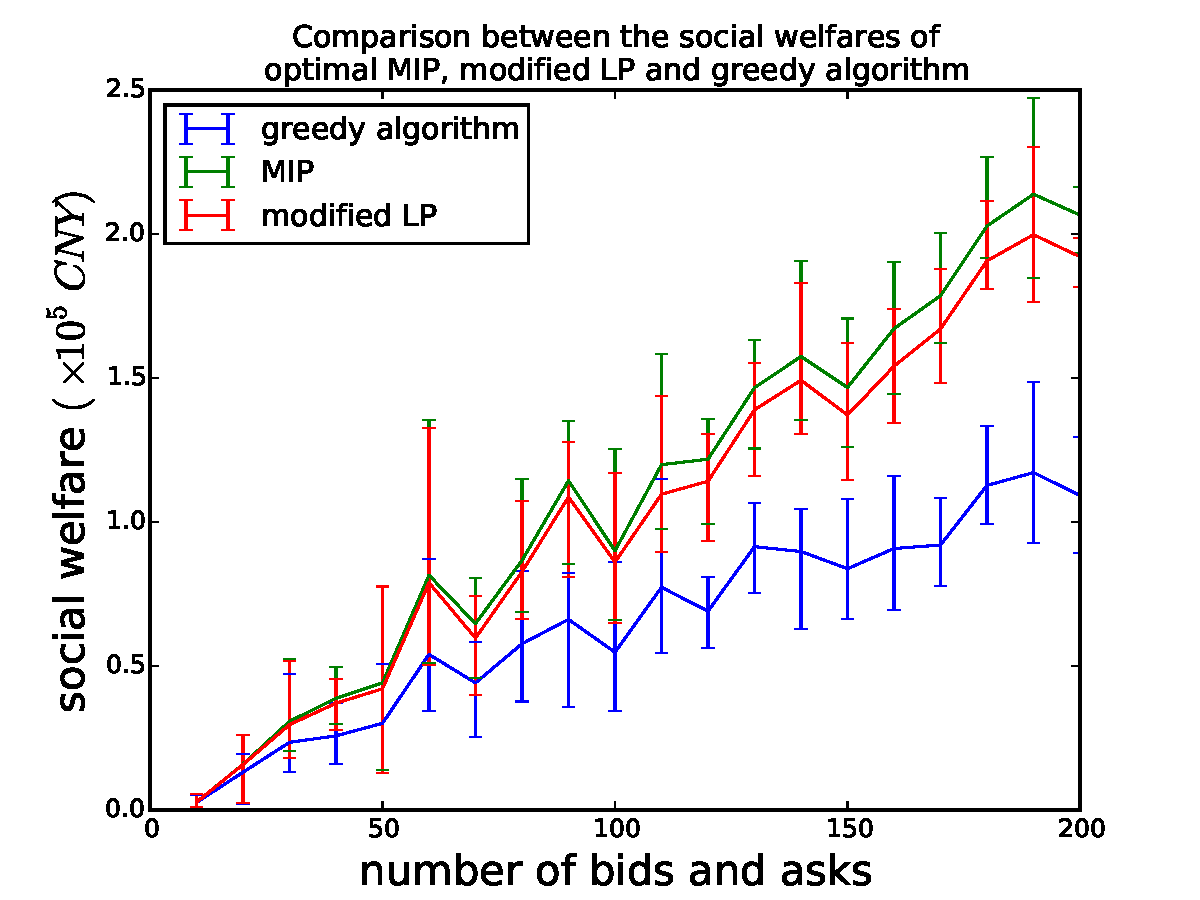
\includegraphics[scale=0.45]{compare.pdf}
	\label{fig:compare}
\end{figure}
\begin{figure}[!ht]
	\centering
	\caption{Comparison between the volumes of MIP and the greedy algorithm}
	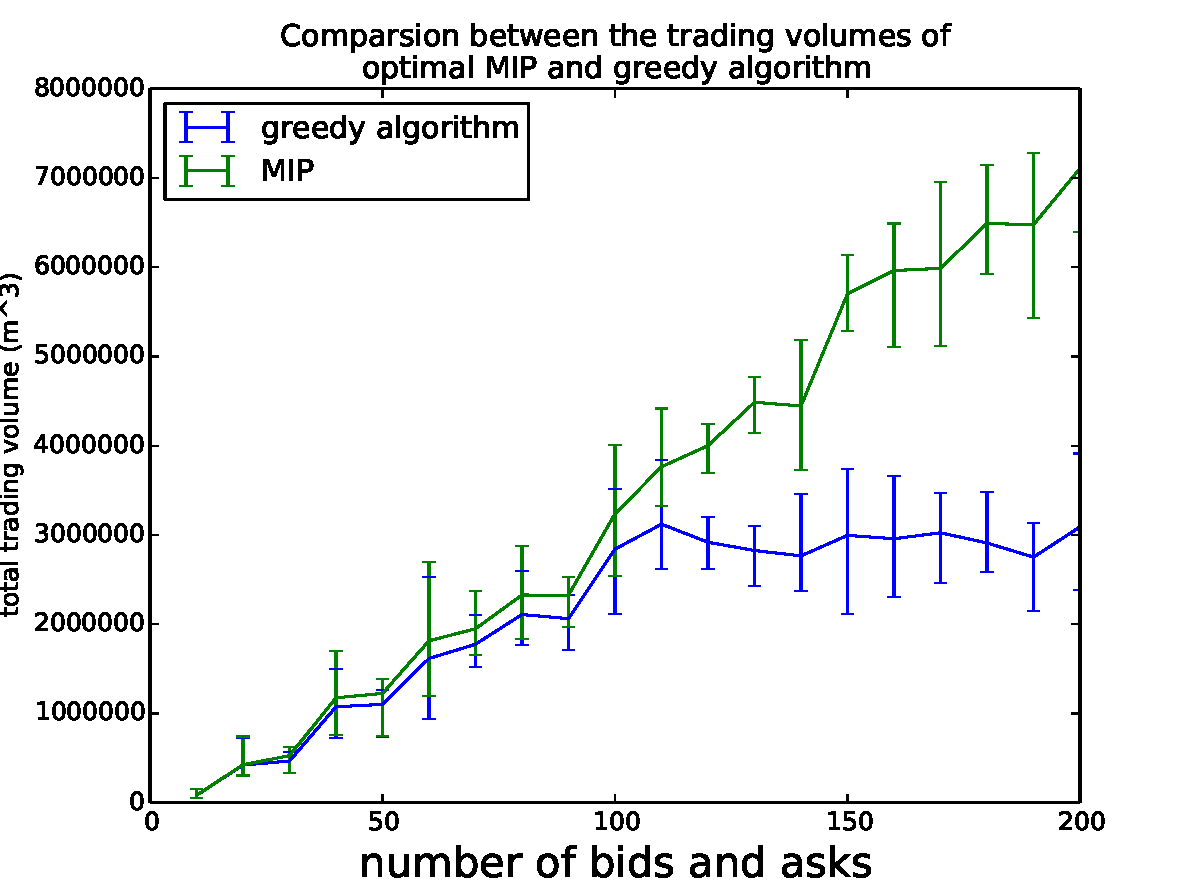
\includegraphics[scale=0.45]{compvol.pdf}
	\label{fig:compvol}
\end{figure}
%\begin{figure}[!ht]
%	\begin{minipage}[t]{0.45\linewidth}
%		\centering
%		\includegraphics[width=1.5in]{newmoney}
%	\end{minipage}%
%	\begin{minipage}[t]{0.45\linewidth}
%		\centering
%		\includegraphics[width=1.5in]{newtime}
%	\end{minipage}
%	\caption{Results on sparse graphs. Comparison between MIP and LP. The lines connect medians.}
%	\label{fig:comp0}
%\end{figure}
%
%\begin{figure}[!ht]
%	\begin{minipage}[t]{0.45\linewidth}
%		\centering
%		\includegraphics[width=1.5in]{money}
%	\end{minipage}%
%	\begin{minipage}[t]{0.45\linewidth}
%		\centering
%		\includegraphics[width=1.5in]{time}
%	\end{minipage}
%	\caption{Results on fully connected graphs. Comparison between MIP and LP. The lines connect medians.}
%	\label{fig:comp}
%\end{figure}
%Fig. \ref{fig:comp0} shows the results for the first connection setup.

Our experimental result suggests that when the connections are sparse (generated by the instance generator), MIP can easily scale to 5000 nodes. LP runs even faster, but with slightly less social welfare due to our modification.

Fig. \ref{fig:comp} shows the results for the complete graph setup.
The welfare of MIP is significantly better than the algorithm based on LP both on social welfare and transaction volume.
However, as for running time, LP is much faster than MIP.
So, when data size is not too large (for example, the current market size), MIP can efficiently return optimal solution.
However, when market becomes larger, the LP algorithm (and its rounding alternatives) can be a good alternative choice.


\section{Conclusion and Future Works}
In this paper, we introduced and studied a new type of market called water right trading market. There are certain unique features that distinguish this market from previously studied double sided markets: (1) trades are restricted by geographical factors such that not each pair of buyer and seller can trades; (2) there are transaction thresholds, such that a small trade is not acceptable. These features trigger new computation problems. We study these problem from both theoretical and experimental perspective.

For the theoretical part, we show most related computational problems are {\sc NP-hard}, or cannot be efficiently approximated.
We use an MIP to solve the most general case and propose several polynomial time algorithms when the underlying graphs have special structures.
For the experimental part, our results confirm that our MIP and LP can work particularly well in general graphs. Surprisingly, the MIP algorithm is even much faster than the polynomial time algorithms on special graphs such as lines and trees.

There are quite a few exciting future directions. We briefly describe three major ones. Firstly, it is perhaps the most important to put our solutions into practice. We are currently in touch with the government in charge and making positive progresses. Secondly, we want to investigate the case where the center specified the prices for each trade and in particular, study how one should trade off between efficiency and budget deficit. Last but not least, we wish to incorporate data into the design, for example, to come up with a better model for geographical connectivities.
\bibliographystyle{abbrv}
\bibliography{water}
\end{document}
